\section{Result}

Having obtained the posterior distribution of the parameters, we can calculate their means, 95\% credible interval, and the probabilities of them being different from 0 (See \autoref{tab:hierarchical_estimate}). Having an legislature improves the positivity in regime-dissident interaction by 0.48 point along the Goldstein scale, and we are 89\% certain that this effect is truly positive. In addition, a party dictatorship improves the interaction by 3.09, a substantively significant effect.

While this model result provides some support for the moderation effect of authoritarian legislature on political violence, the size of the substantive effect is quite small given that regime-dissdent interactions typically scatter along a 10-unit spectrum on the Goldstein scale (-10 to 0). Since our model allows full flexibility in the country-year and country intercepts, it reveals that much of the variation in violence is captured in these group-specific intercepts. This suggests that the included set of co-variates, which is standard in the literature, have not fully explained the pattern of violence.

\begin{table}[H]
\centering
\begin{tabular}{rrrrrr}
  \hline
 & mean & 2.5\% & 97.5\% & Pr( $>$ 0) & Pr( $<$ 0) \\ 
  \hline
legislature & 0.48 & -0.29 & 1.25 & 0.89 &  \\ 
  log(GDP percap) & -0.39 & -1.31 & 0.52 &  & 0.81 \\ 
  log(GDP) & 0.37 & -0.19 & 0.92 & 0.91 &  \\ 
  resource (\%GDP) & -0.01 & -0.04 & 0.02 &  & 0.78 \\ 
  military exp (\%GDP) & -0.04 & -0.27 & 0.19 &  & 0.63 \\ 
  regime duration & 0.02 & -0.03 & 0.08 & 0.78 &  \\ 
  military regime & 2.10 & -1.79 & 5.84 & 0.86 &  \\ 
  personal regime & 1.60 & -1.65 & 4.89 & 0.83 &  \\ 
  party regime & 3.09 & -0.10 & 6.31 & 0.97 &  \\ 
   \hline
\end{tabular}
\caption{Hierarchical model parameter estimates}
\label{tab:hierarchical_estimate}
\end{table}

\begin{figure}[ht]
    \centering
    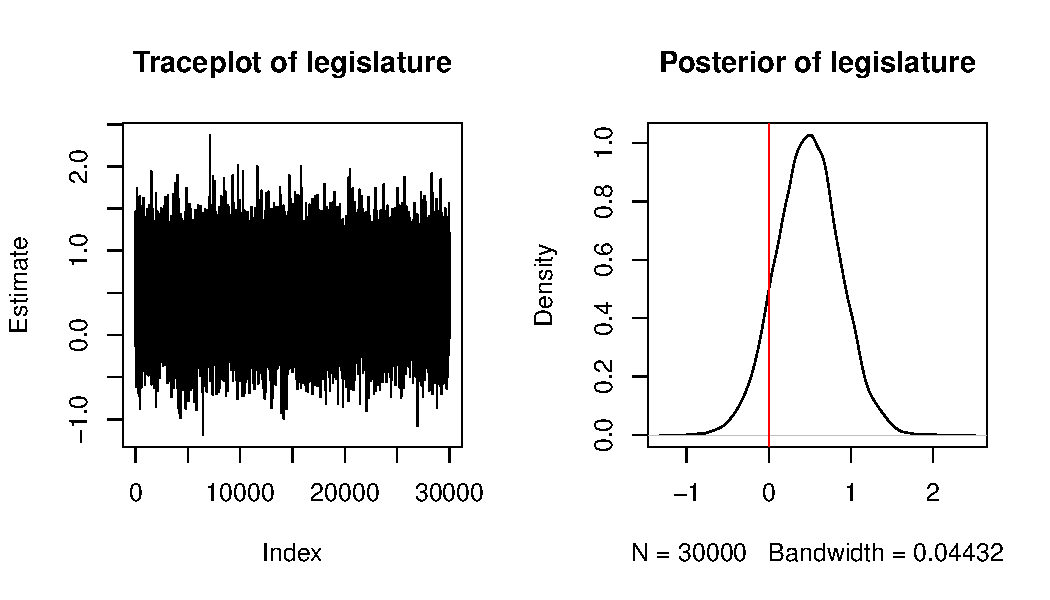
\includegraphics[width=\textwidth]{../fig/mcmc_legis}
    \label{fig:mcmc_legis}
\end{figure}
